\chapter{Обзор существующих решений для генерации персонажа D\&D}

Среди многих таких решений для игроков, которых великое множество, наибольшей популярностью пользуются в основном те, которые обладают наибольшей функциональностью и гибкостью настройки (обычно такие генераторы могут создать полностью случайного персонажа или позволить, при необходимости, тонко настроить его). Такие генераторы хорошо подходят как для новичков, которым нужно быстро сгенерировать персонажа, который будет пригоден для освоения правил игры, так и для опытных игроков, которые любят прорабатывать своего персонажа досконально. Также такие генераторы отлично подходят и для Мастеров, которым нужно использовать много второстепенных персонажей и для которых также не нужно подробно прорабатывать второстепенных персонажей.

Ниже представлены самые популярные из таких решений, которые заслуживают наибольшего внимания:

\begin{enumerate}
    \item D\&D Beyond.
    \item AideDD.
    \item Dungeon Master’s Vault.
    \item Fast Character Genarator.
    \item Javascript DDNext Character Generator.
    \item Levi Blodgett’s Character Generator.
    \item MPMB’s DnD 5e Character Tools.
    \item Ninetale Character Builder.
    \item Roll20 Charactermancer.
    \item 5e Companion App.
\end{enumerate}

Все они представляют из себя Web-приложения или мобильные приложения, но каждое из них имеет свои особенности.

Основное назначение генератора персонажа заключается в том, чтобы помочь игроку в создании своего игрового персонажа с определенными характеристиками и снаряжением, который был бы готов к игре. Такой генератор характерен для многих тяжёлых систем, позволяет автоматически рассчитывать вторичные характеристики и избавляет игрока от обращения в дополнительные источники и сокращает выборы, отсекая недоступные опции при создании персонажа (с учётом предыдущих этапов его создания). Генераторы такого типа могут быть как опциональными (и предназначаться только для какого-то отдельного этапа создания персонажа --- например, механизация выбора жизненного пути), так и основным способом создания в системе.

Базовый набор характеристик, которые позволят сгенерировать и рассчитать конструктор персонажа выглядит следующим образом:

\begin{enumerate}
    \item Выбор расы персонажа.
    \item Выбор класса персонажа.
    \item Генерация значений 5 базовых характеристик: Сила, Телосложение, Ловкость, Интеллект, Мудрость, Харизма.
    \item Расчет значений для ряда побочных характеристик: класс защиты и хит-поинтов персонажа (на основе базовых характеристик).
    \item Выбор снаряжения на основе ранее выбранных игроком характеристик.
\end{enumerate}

Опционально в некоторых генераторах встречаются следующие возможности:

\begin{enumerate}
    \item Импорт листа персонажа в PDF-файл.
    \item Создание собственных пользовательских классов или материалов.
\end{enumerate}

\section{D\&D Beyond}

Это официальный цифровой инструмент, предлагаемый Wizards of the Coast, издателем Dungeons \& Dragons. Web-сайт предлагает цифровые копии своих книг (данная функция доступна за деньги), в том числе три основных книги для 5-го издания (Руководство игрока, Руководство мастера подземелий и Руководство монстров), а также собственные приключения Волшебника.

D\&D Beyond также имеет инструмент для создания персонажей, который значительно упрощает процесс, и даже предоставляет цифровой лист персонажа для этого персонажа после его создания. В качестве альтернативы присутствует возможность скачать листы персонажей с возможностью заполнения формы и заполнить их самостоятельно. Интерфейс генератора приведен на рис.~\ref{fig:beyond}.

Однако, отличительная особенность и лучшая функция D\&D Beyond --- это огромный индекс всех официальных заклинаний, оружия, предметов и монстров на сайте. Также приложение позволяет просматривать любые домашние заготовки, которые можно использовать в кампании.

D\&D Beyond пожалуй, самый известный справочный сайт для D\&D 5е. Только часть контента и материалов бесплатны, но конструктор персонажей доступен с бесплатной учетной записью.

Это очень гибкая система с множеством шагов настройки и дополнительных систем, включая три различных метода генерации характеристик. Причем, после создания множество исходных материалов, которые использовались для создания, можно использовать для дальнейшего заполнения персонажа.

\begin{figure}[H]
    \centering
    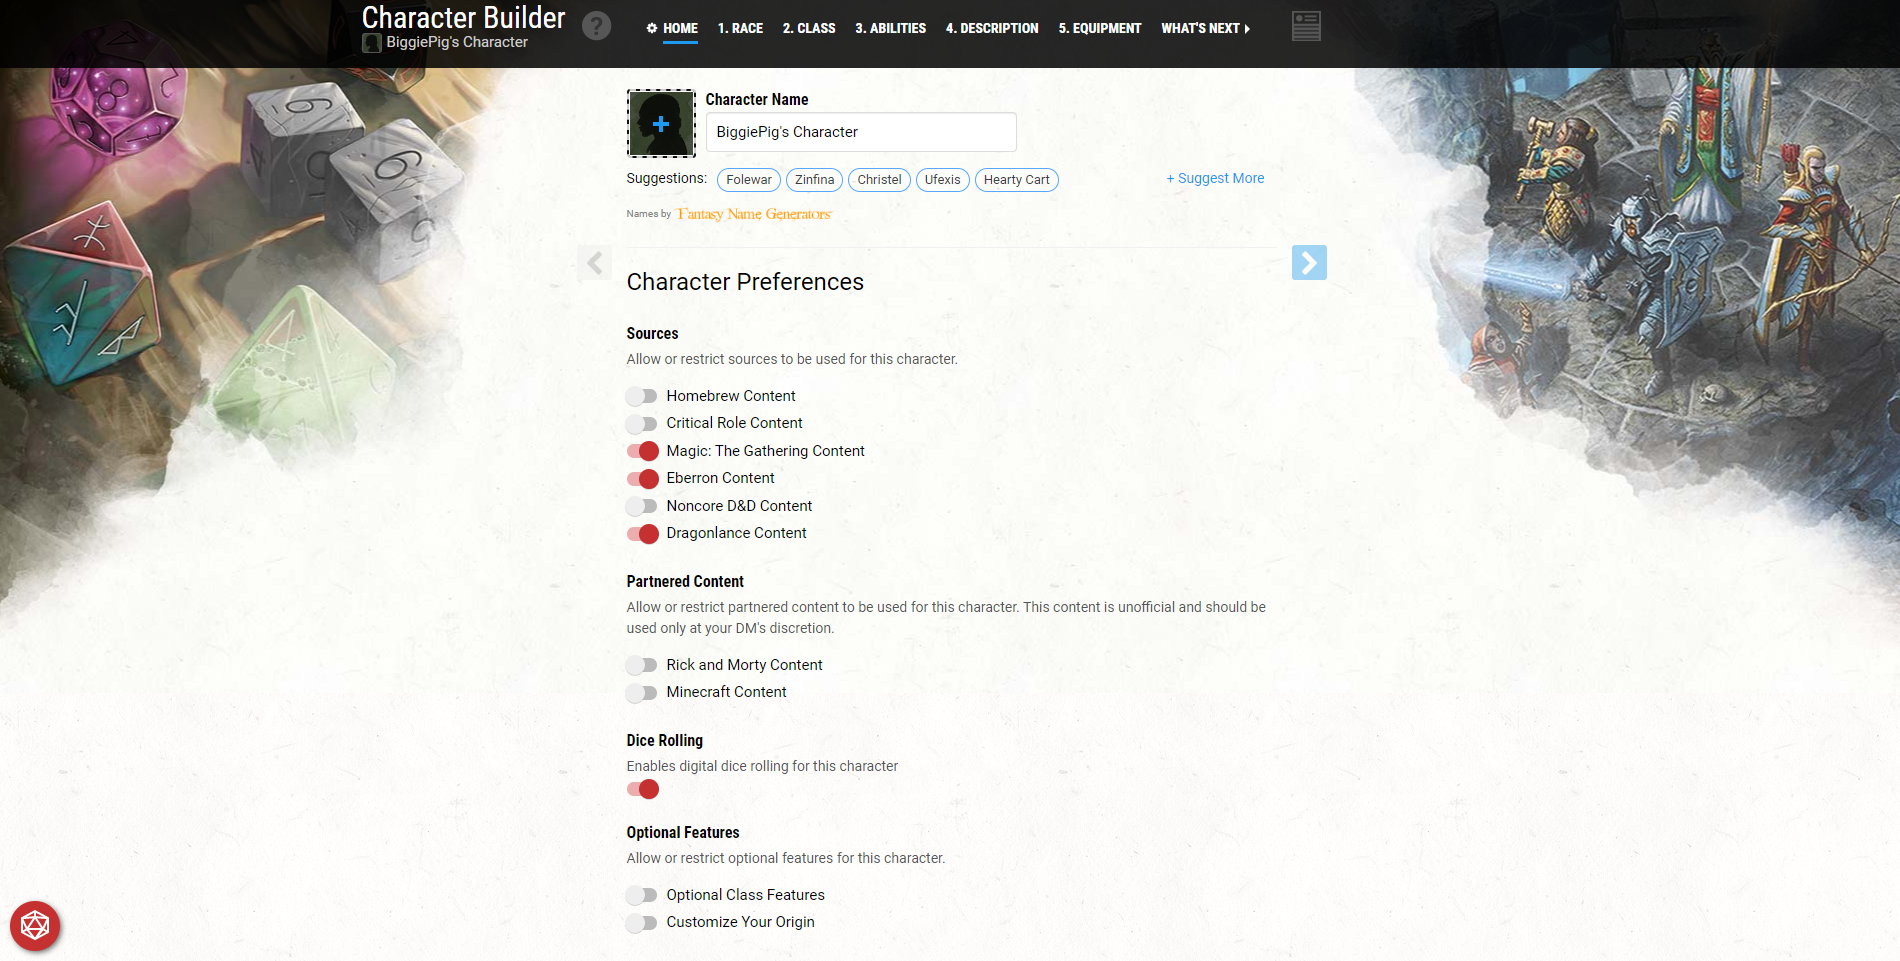
\includegraphics[scale=0.3]{DnD_Beyond.png}
    \caption{Интерфейс генератора персонажа D\&D Beyond~\cite{beyond}.}
    \label{fig:beyond}
\end{figure}

Каждая характеристика или элемент на странице имеет ссылку на более подробные описания и пояснения, избавляя от необходимости постоянно листать книги правил, чтобы узнать, что делает тот или иной предмет, или какие бонусы можно получить от статистики.

Можно не только создать персонажа с настраиваемыми параметрами на каждом этапе и создать пользовательские характеристики, используя один из трех методов (4d6 best 3, стандартный массив или покупка очков), но и получившийся в результате лист персонажа имеет доступ к справочным материалам D\&D Beyond. 

Любой шат или предмет на листе персонажа можно расширить, чтобы дать его полное описание, что может быть очень полезно. Кроме того, на листе есть встроенный ролик для игры в кости, который можно использовать во время игры.

Основным недостатком является то, что это не самый лучший сайт для быстрой случайной генерации персонажей; необходимо пройти каждый шаг, который может стать утомительным для мультиклассовых персонажей.

\section{AideDD}

AideDD --- дна из лучших систем для новичков в игре. Конструктор персонажей AideDD разбивает процесс создания персонажа на очень простые шаги, которые значительно упрощают выбор, связанный с созданием персонажа. Но он не только прост в использовании, но и кажется глубоким; только у нескольких онлайн-строителей есть все заклинания в справочнике D\&D, в том числе у этого.

К недостаткам можно отнести то, что доступны только некоторые расы или классы, и мало пользовательских функций, которые для компенсации этого.

Генератор прост в использовании, и можно экспортировать созданного персонажа в виде XML-файла или в Официальный лист персонажа D\&D 5e.

Внешний вид генератора представлен на рис.~\ref{fig:aidedd}.

\begin{figure}[H]
    \centering
    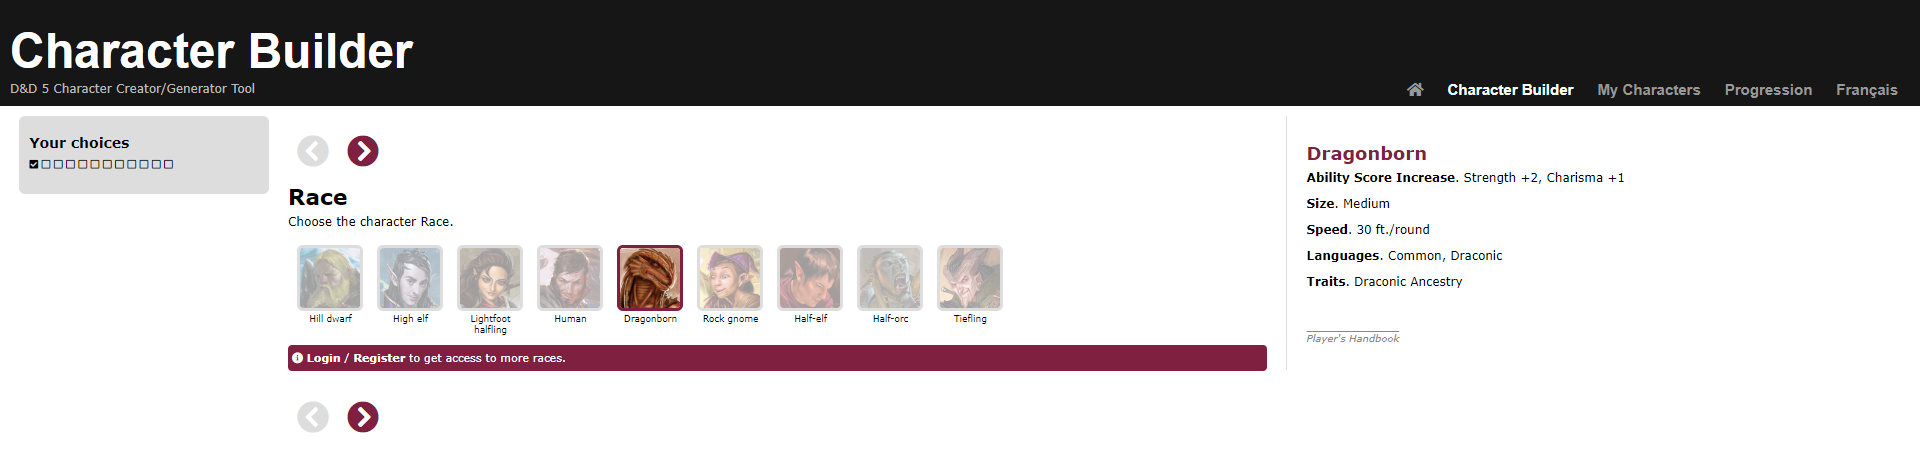
\includegraphics[scale=0.3]{Aidedd.png}
    \caption{Интерфейс генератора персонажа Aidedd Character Builder~\cite{aidedd}.}
    \label{fig:aidedd}
\end{figure}

\section{Dungeon Master’s Vault}

Этот генератор не так известен, как D\&D Beyond, но Хранилище Мастера Подземелий имеет все основные достоинства этой системы и очень мало ее недостатков. Основным преимуществом является его гибкость, позволяющая случайным образом генерировать персонажей и использовать их в качестве более практичного и тщательного ресурса для создания.

\begin{figure}[H]
    \centering
    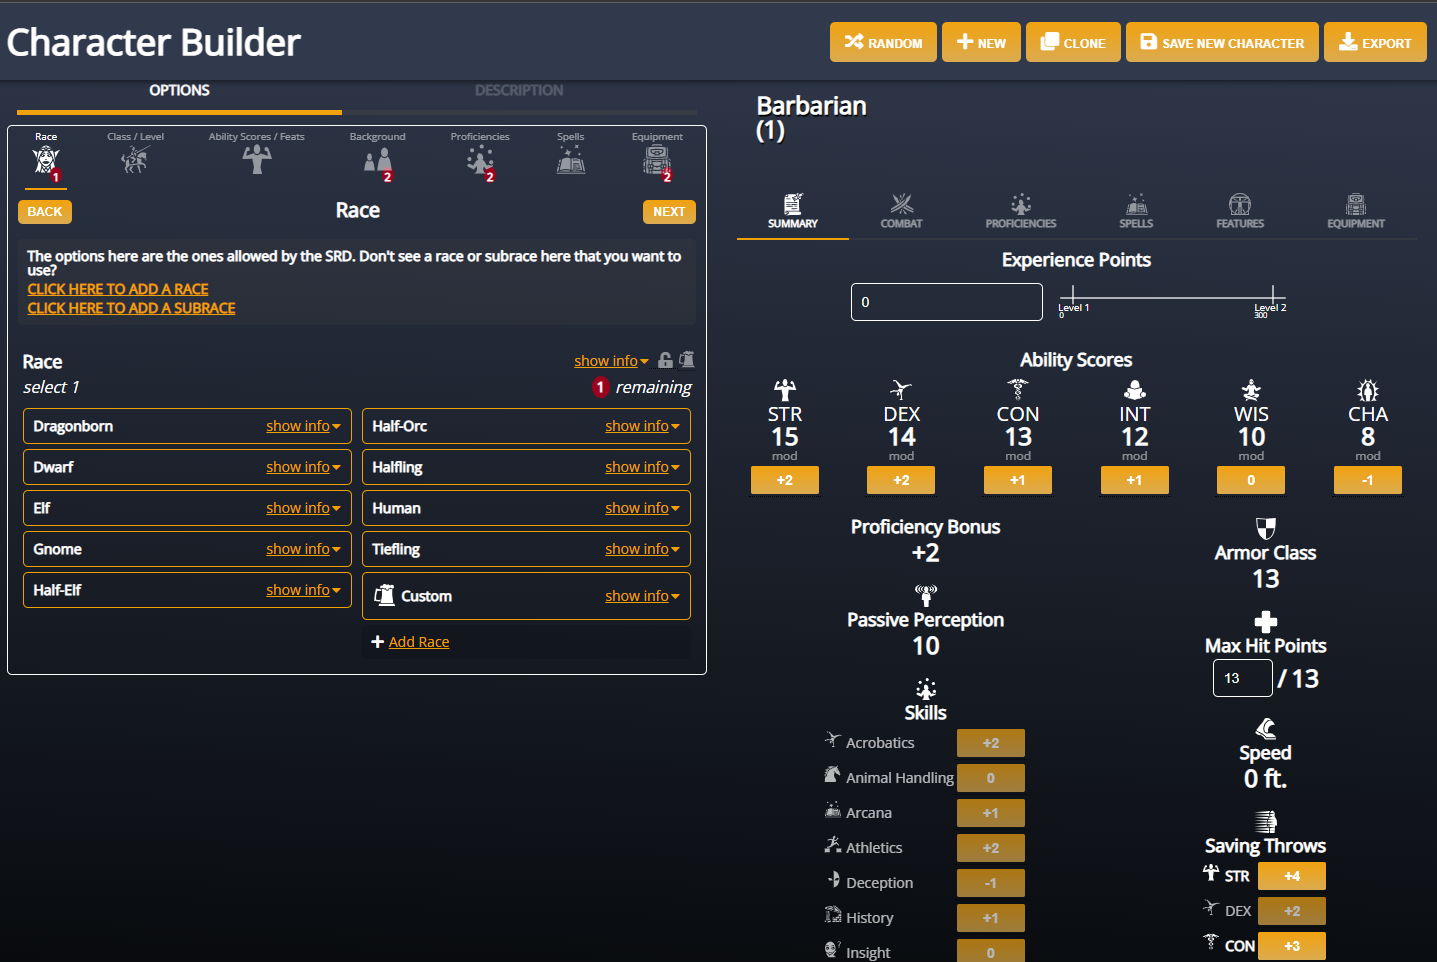
\includegraphics[scale=0.4]{Dungeon_Master's_Vault.png}
    \caption{Интерфейс генератора персонажа Dungeon Master's Vault~\cite{dmv}.}
    \label{fig:DM_Vault}
\end{figure}

Генератором поддерживается создание мультиклассовых персонажей более высокого уровня, для которых сайт сообщит о том, является ли персонаж легальным для Лиги Авантюристов, у которой есть свои собственные правила создания персонажа в D\&D 5e.

Также ресурс позволяет сгенерировать все необходимое для начала игры, что очень полезно для Мастеров. Предусмотрены генераторы для: городов D\&D 5e, NPC D\&D 5e, имен D\&D 5e, слухов D\&D 5e и плакатов розыска D\&D 5e.

У данного генератора есть недостаток, который заключается в том, что генератор не охватывает всесторонне все заклинание, класс и подкласс, но такую недостающая информация, можно ввести вручную с помощью простой в использовании пользовательской функции.

\section{Fast Character Genarator}

При самой быстрой настройке пользователю не нужно делать выбор чего-либо самостоятельно; приложение может сделать всю работу, что является наиболее подходящим для новых игроков, которым нужен персонаж, на котором они могли бы тренироваться, изучая основы игры.

Также это может помочь, если пользователь --- опытный игрок, просто стремящийся по-настоящему отойти от своих обычных наклонностей и желающий получить персона, который будет получен при помощи рандомайзера.

\begin{figure}
    \centering
    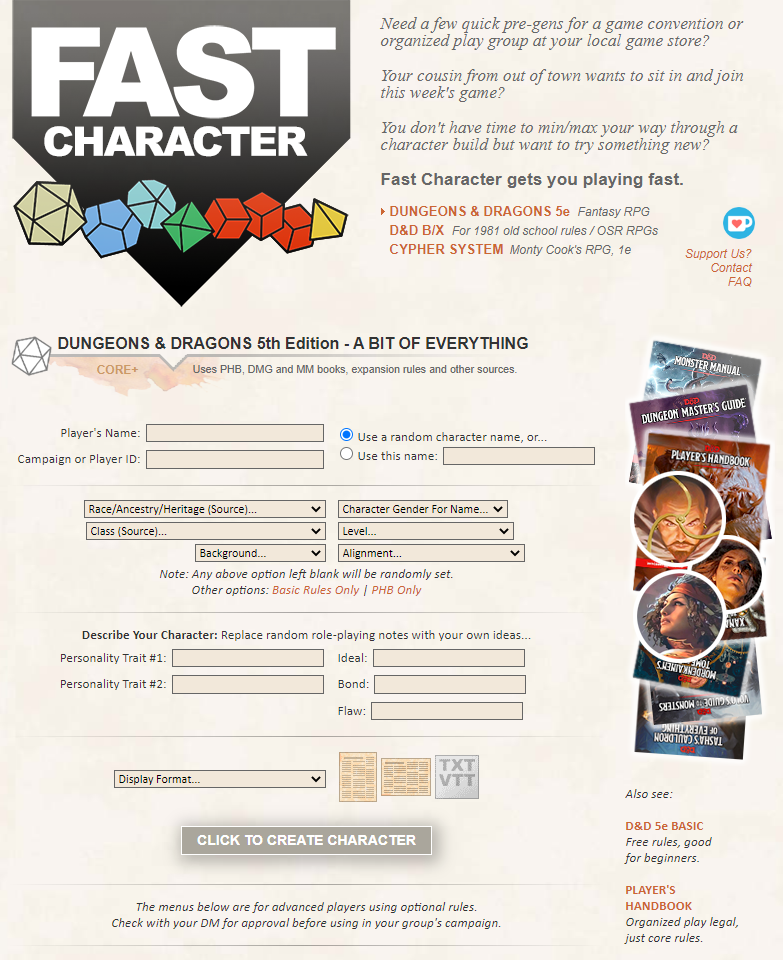
\includegraphics[scale=0.4]{Fast_character.png}
    \caption{Интерфейс генератора персонажа Fast Character Builder~\cite{fast_char}.}
    \label{fig:fast_char}
\end{figure}

Самостоятельное создание персонажа также происходит довольно быстро; выбор осуществляется с помощью простых и интуитивно понятных меню с выпадающим списком. После того, как генерация закончена, пользователю предлагается выбрать один из нескольких вариантов отображения готового листа персонажа. 

Сайт предлагает только некоторые подклассы, и большим недостатком этого конструктора является то, что он также не поддерживает создание мультиклассовых персонажей. Назначение характеристик представляет из себя более сложный процесс в том случае, если пользователь собирается производить все настройки самостоятельно.

Это лучший конструктор для мастеров, которым нужен быстрый персонаж с несколькими заданными деталями. 

Игрокам обычно нужен один персонаж, чтобы пройти кампанию. Мастерам подземелий их нужно много, чтобы заполнить сессию. В этом основное достоинство быстрого конструктора для мастеров.

\section{Javascript DDNext Character Generator}

Данный генератор предоставляет огромное количество опций и настроек, которые позволяют игроку осуществлять полный контроль над созданием своего персонажа.

\begin{figure}
    \centering
    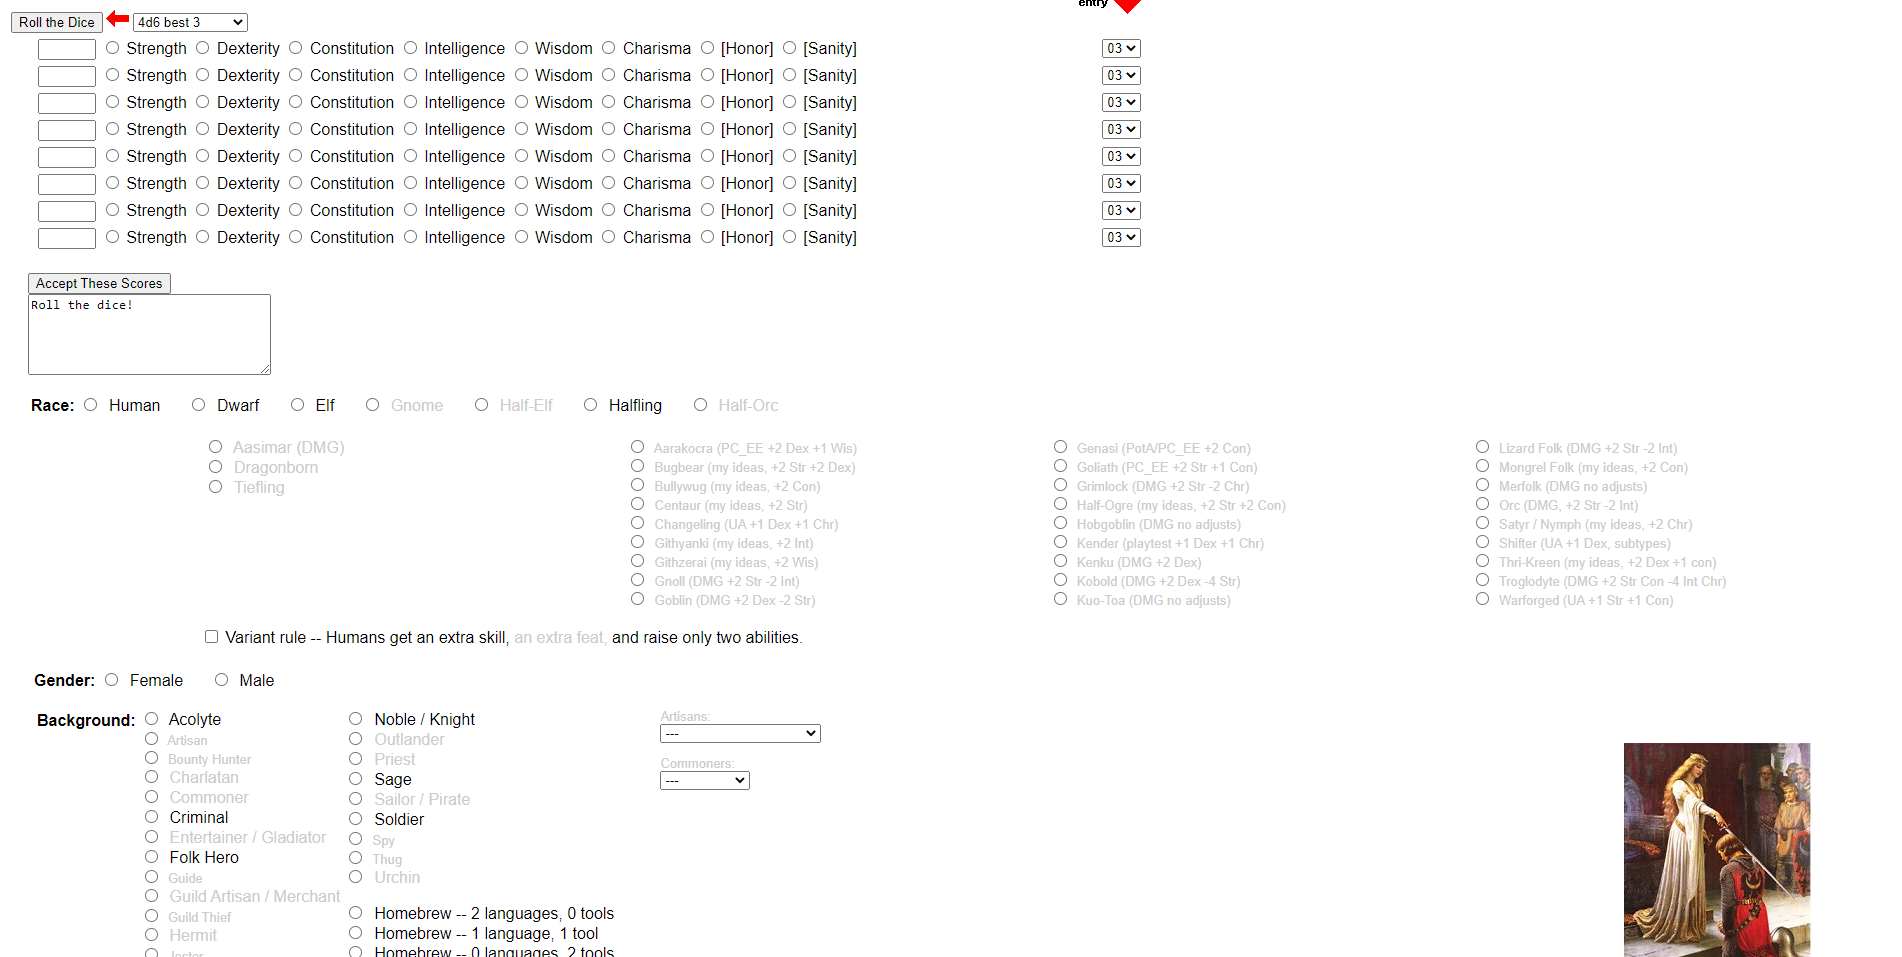
\includegraphics[scale=0.3]{DDNext.png}
    \caption{Интерфейс генератора персонажа Javascript DDNext Character Generator~\cite{ddnext}.}
    \label{fig:ddnext}
\end{figure}

В этом конструкторе есть множество способов, которыми можно рассчитать свою статистику (3d6, 4d6 лучшие 3, 5d6 лучше 3, простой ввод, стандартный массив, неэлитный массив), а также несколько вариантов пользовательских настроек, от показателей характеристик до снаряжения. 

Также, конструктор позволяет создавать персонажей более высокого уровня 5e, а также мультиклассовых персонажей. Но этот конструктор не предлагает все варианты в D\&D, как и большинство генераторов здесь,, и не всегда у пользователя есть возможность ввести свои собственные настройки. 

Пользовательский интерфейс также может быть немного запутанным; есть полезные указатели. Данный конструктор рекомендует определенные варианты по сравнению с другими в зависимости от того, что выбирает пользователь.

Это отличный конструктор для игры с параметрами персонажа, но он создает <<лист>> персонажа только в виде списка текста, что не является быстрой генерацией.

\section{Levi Blodgett’s Character Generator}

Данный конструктор персонажа собирает полностью редактируемый лист персонажа D\&D 5e. Пользователь имеет возможность точечно настроить его по своему усмотрению, а после окончания сохранить в формате PDF.

\begin{figure}[H]
    \centering
    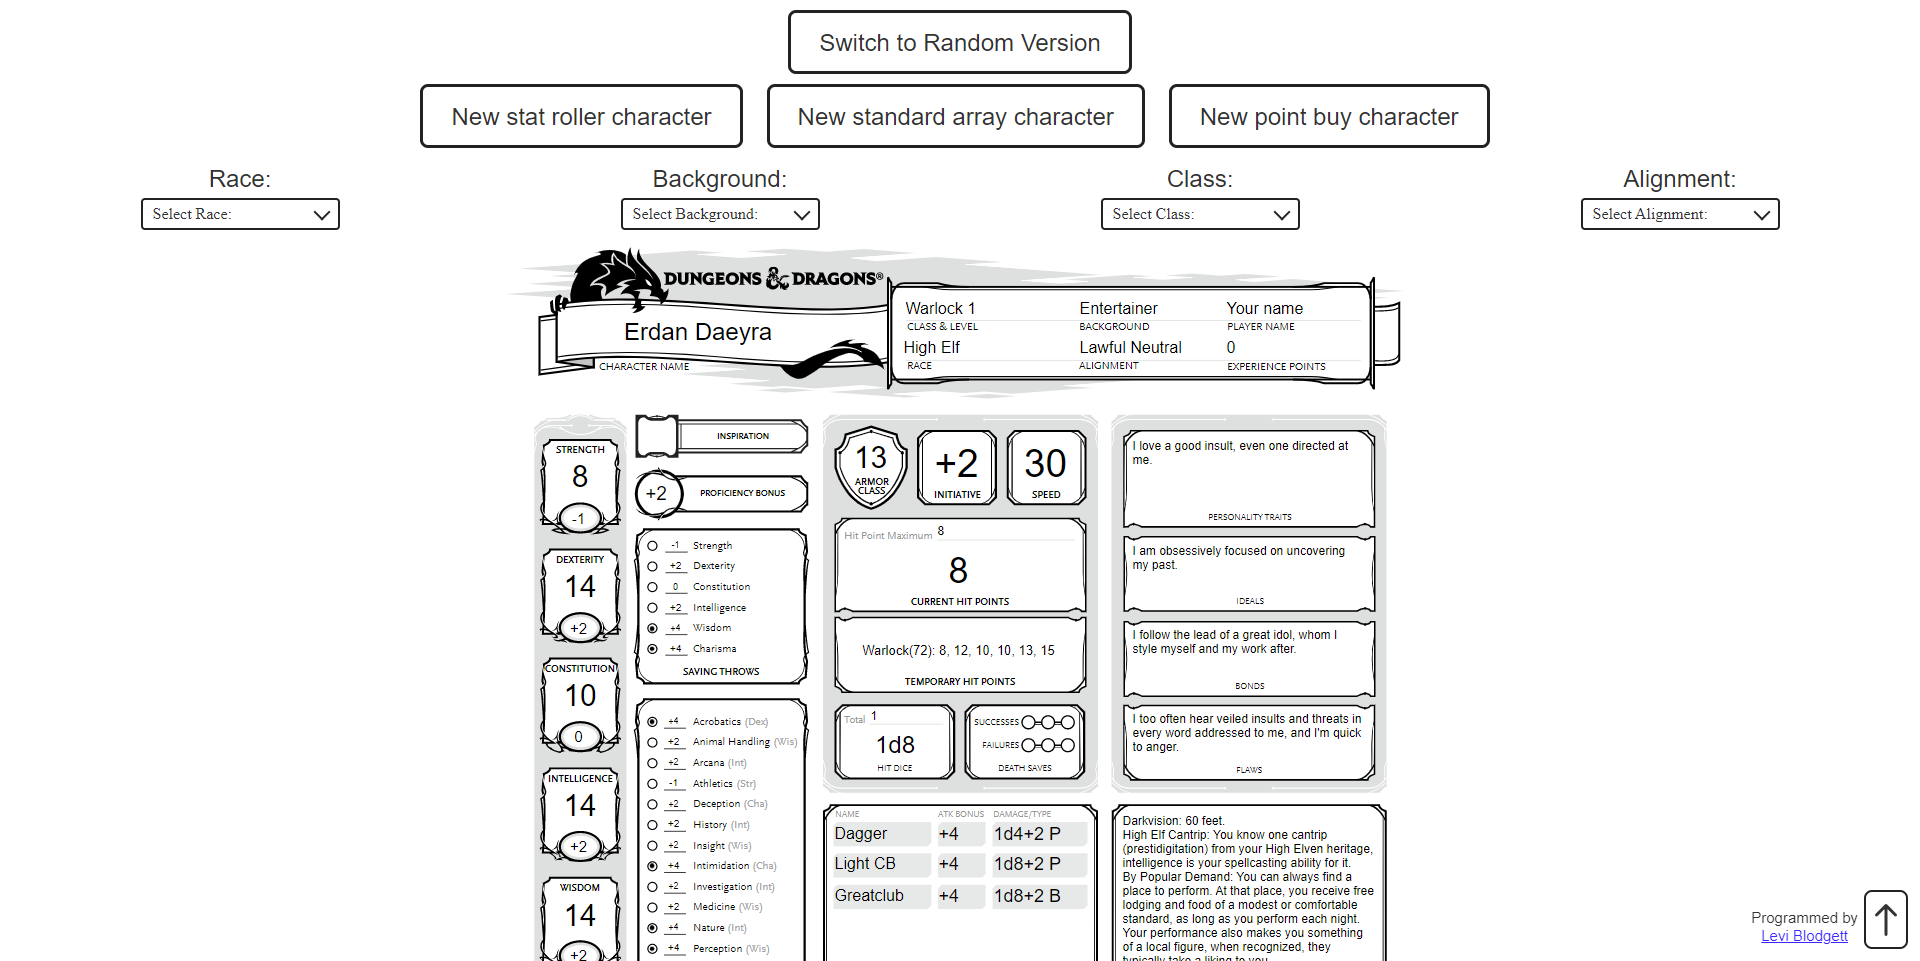
\includegraphics[scale=0.3]{Levi_Blodgett.png}
    \caption{Интерфейс генератора персонажа Леви Блоджетта~\cite{levi}.}
    \label{fig:blodgett}
\end{figure}

Этот конструктор хорош тем, что пригоден для быстрой генерации случайных персонажей, как и конструктор, описанный выше. Присутствует возможность не только создавать по-настоящему случайных персонажей (или фильтровать по определенным классам, расам или предыстории), но и использовать <<Логическую версию>>, которая создает персонажа на основе случайно выбранных характеристик, которые взаимосвязаны между собой.

Генератор случайных чисел достаточно быстр, а для быстрого персонажа это один из лучших конструкторов. Но если пользователь желает создать своего собственного персонажа, то предоставляется возможность редактировать лист вручную.

Есть возможность генерировать символы выше уровня 1, только редактируя лист напрямую; генератор случайного персонажа при этом не работает.

\section{MPMB’s DnD 5e Character Tools}

MorePurpleMoreBetter также является примером обширного конструктора персонажей. Этот конструктор в действительности состоит из нескольких взаимосвязанных конструкторов, которые работают вместе через PDF-файлы MPMB.

\begin{figure}[H]
    \centering
    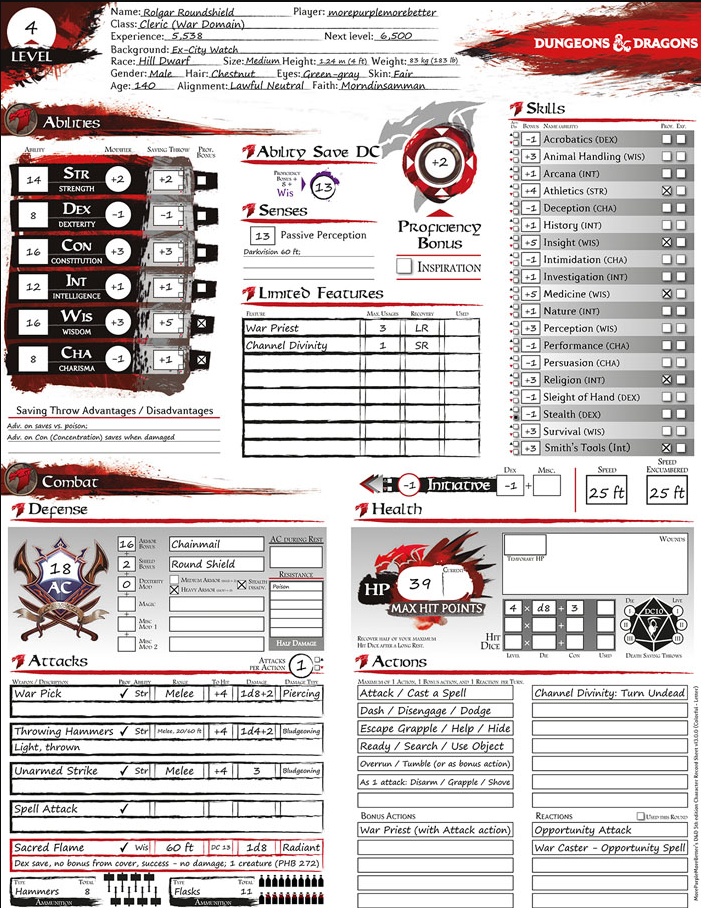
\includegraphics[scale=0.5]{MPMB.png}
    \caption{Интерфейс генератора персонажа MorePurpleMoreBetter~\cite{mpmb}.}
    \label{fig:mpmb}
\end{figure}

Данный продукт, в отличие от остальных, является платным. Стоимость подписки составляет 1 доллар в месяц.

С использованием Java Script конструктор персонажей включает в себя листы от улучшенного листа персонажа D\&D 5e и листа  заклинаний до подробных листов для компаньонов и многое другое.

Хотя этот конструктор персонажей ограничен контентом SRD, он поддерживает полную настройку и на сегодняшний день является одним из лучшик конструкторов персонажей, когда надо настроить лист персонажа.

\section{Ninetale Character Builder}

Конструктор персонажей Ninetale не так обширен, как MPMB, но он подходит для создания быстрых и простых персонажей. 

Отличительной особенностью данного генератора является его удобный блок характеристик. Он не генерирует полный лист персонажа, как другие конструкторы, но блок характеристик, который он создает, намного удобнее для мастеров.

К недостаткам этого генератора можно отнести то, что он не очень настраиваемый. Присутствуют ограничения персонажами 1-го уровня, и характеристики могут быть максимально рассчитаны до 15 (не считая расовых бонусов). 

Он также не включает весь опубликованный контент D\&D 5e, что это характерно для большинства создателей персонажей.

\begin{figure}[H]
    \centering
    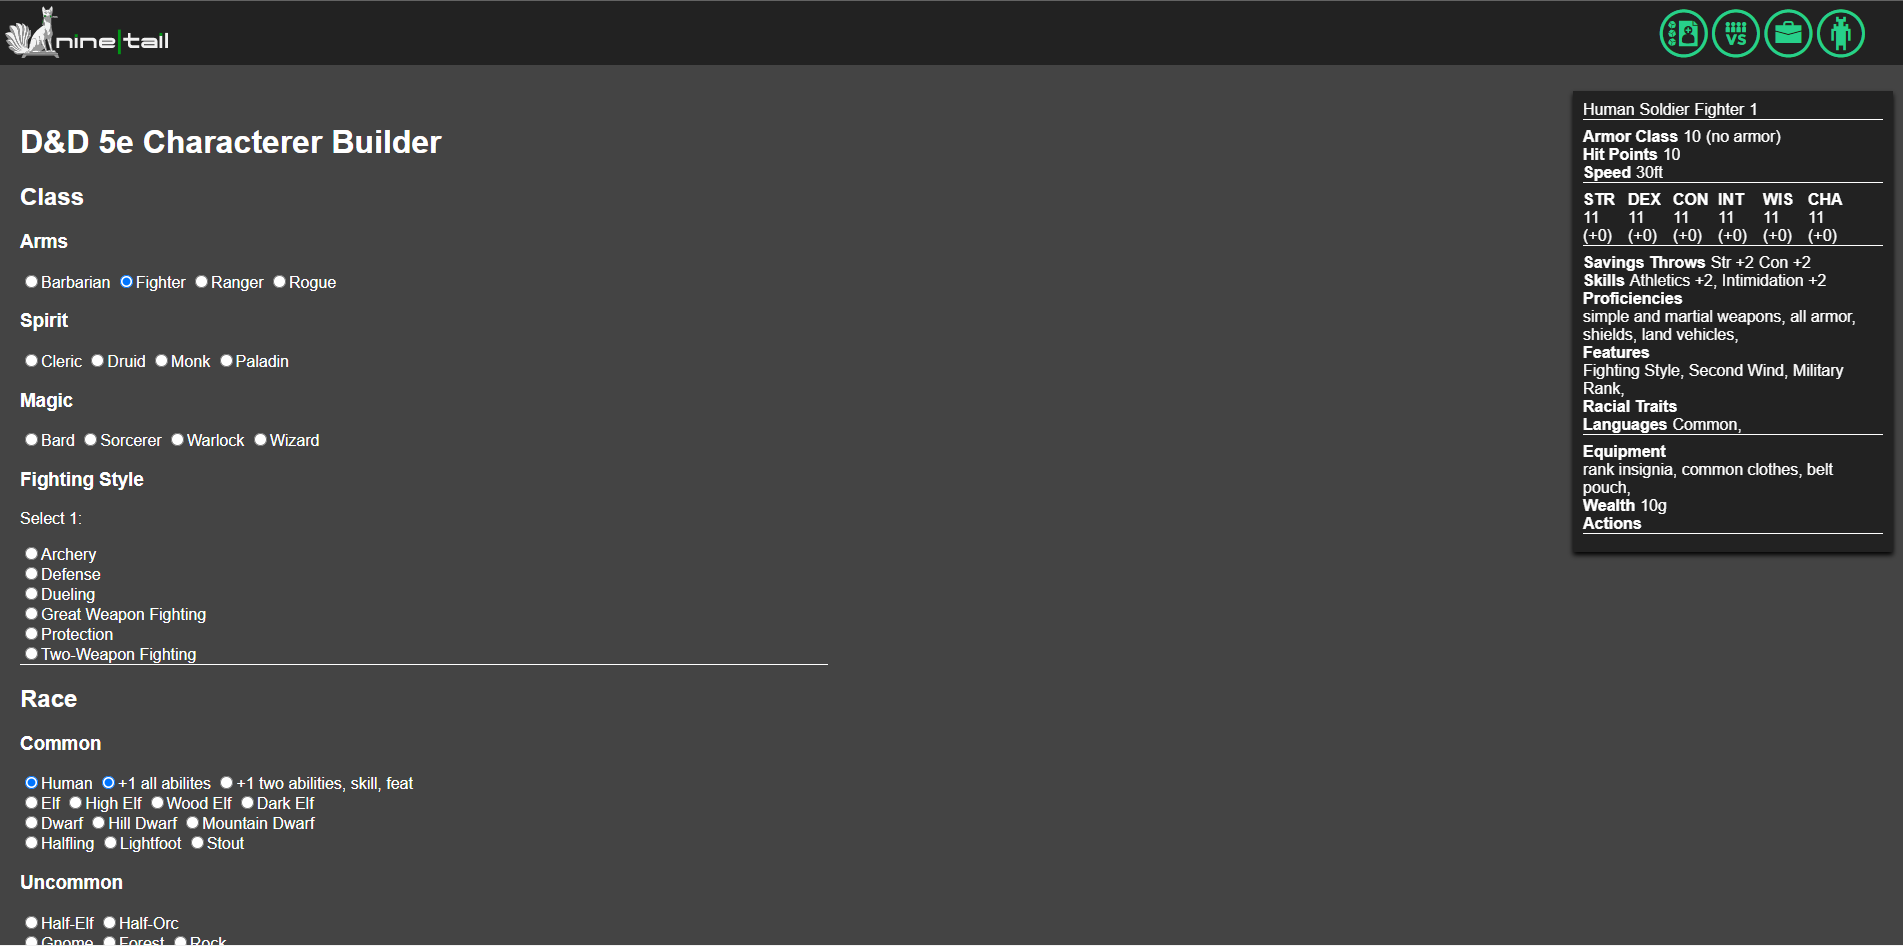
\includegraphics[scale=0.3]{Ninetail.png}
    \caption{Интерфейс генератора персонажа Ninetail~\cite{ninetail}.}
    \label{fig:ninetail}
\end{figure}

Если пользователь хочет быстро создать персонажа, начать с 1-го уровня и погрузиться в свою кампанию 5e, Ninetails является неплохим вариантом. Игроки и мастера подземелий очень легко создают своих персонажей с помощью этого конструктора.

\section{Roll20 Charactermancer}

Сайт Roll20 хорошо известен своими руководствами по правилам D\&D 5e и размещением всевозможных ролевых игр. Полльзователь может присоединиться к ресурсу бесплатно и получить доступ к их 5e конструктору листов персонажей.

\begin{figure}[H]
    \centering
    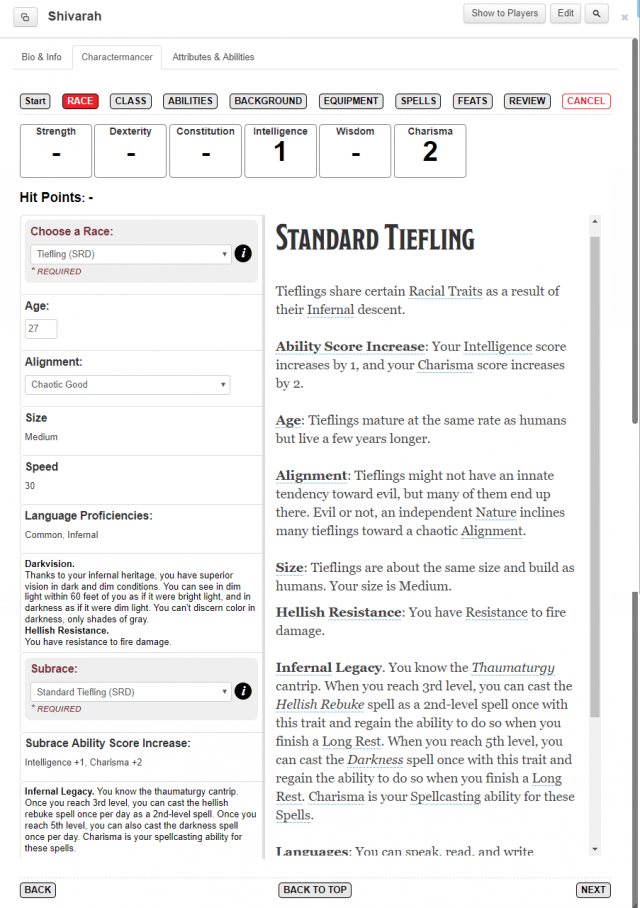
\includegraphics[scale=0.45]{Roll20.png}
    \caption{Интерфейс генератора персонажа Roll20~\cite{roll20}.}
    \label{fig:roll20}
\end{figure}

В данном конструкторе пользователь может напрямую редактировать свой лист персонажа, чтобы создавать не только персонажей первого, но и более высокого уровня и мультиклассовых персонажей, но и персонажей с пользовательским способностями.

И все они напрямую связаны с системой кампании Roll20, что позволяет бросать кости непосредственно с листа или с помощью макроса, который ссылается на этот лист.

Конструктор разбивает процесс создания персонажа на простые вопросы, но что мне действительно нравится, так это то, как он подводит итог вашему персонажу до того, как вы закончите.

У Roll20 также есть то, что он называет Compendium, в котором содержится множество правил и функций D\&D 5e. Это означает, что в большинстве случаев можно просто перетаскивать навыки, предметы, заклинания и многое другое прямо на лист персонажа, не редактируя ничего вручную.

Большим недостатком Roll20 является то, что пока нет возможности экспортировать лист персонажа.

\section{5e Companion}

Также есть приложение 5e Companion. Это единственное достойное приложение, которое предоставляет множество настроек и включает в себя генератор персонажа.

\begin{figure}[H]
    \centering
    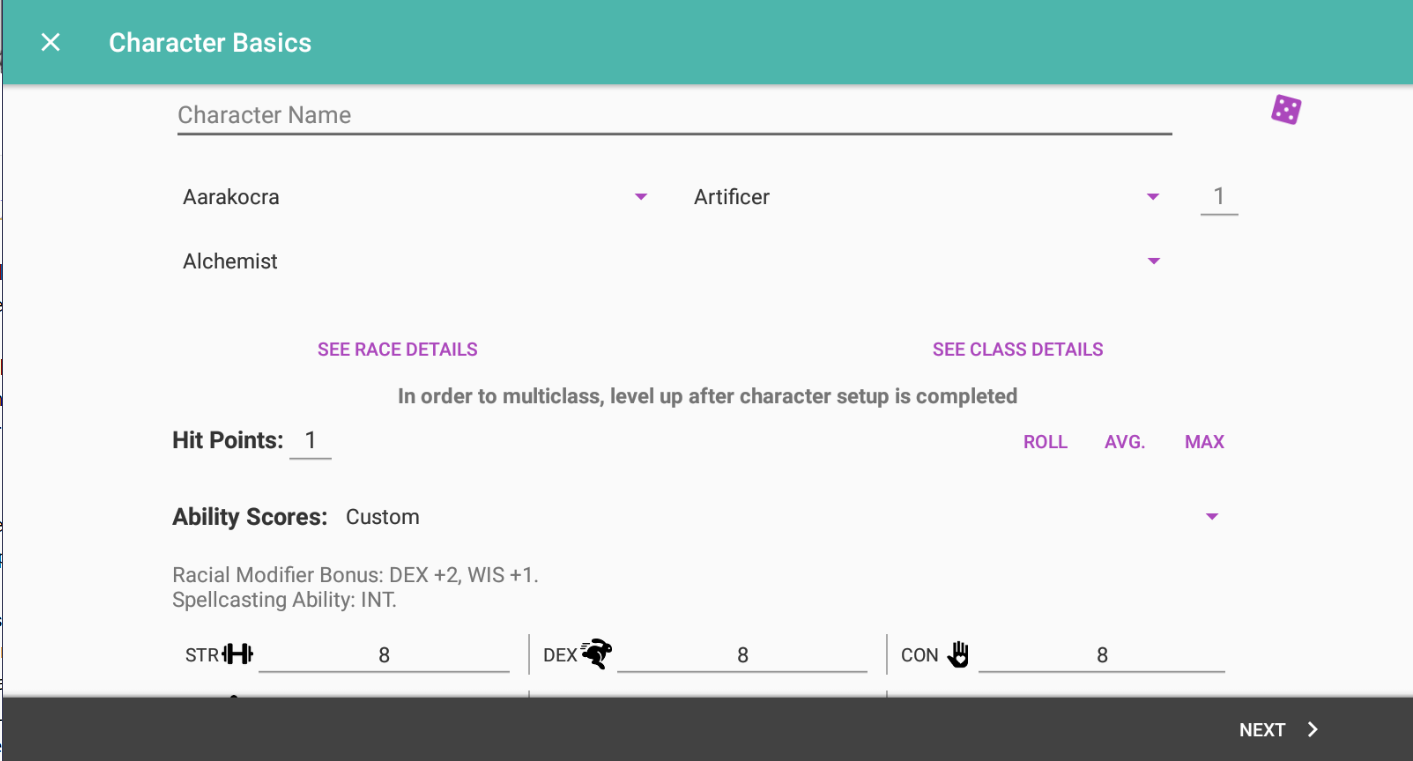
\includegraphics[scale=0.4]{5e_Companion.png}
    \caption{Интерфейс генератора персонажа 5e Companion App~\cite{companion}.}
    \label{fig:5e_companion}
\end{figure}

Приложение предоставляет множество справочной информации. В этом приложении есть не только конструктор персонажей, но и списки заклинаний, монстры и многое другое. 

Конструктор включает в себя почти все, что было бы возможно включить в конструктор персонажей. Он не только содержит весь опубликованный контент, но и позволяет легко добавлять пользовательские способности и заклинания. В данном приложении невозможно случайным образом сгенерировать персонажа так же быстро, как в некоторых других генераторах, но приложение включает рандомизаторы.

У приложения нет возможности экспортировать листы персонажей за пределы приложения. Это делает этот строитель лучшим для справки, но не для игры. 

Тем не менее, для мастеров, которые создают десятки персонажей и действительно могут использовать удобный организованный список, этот конструктор особенно полезен.

Все рассмотренные генераторы персонажей представляют из себя Web-приложения или приложения для телефона, и требуют постоянного подключения к Интернету и наличия у каждого из игроков устройства с выходом в Интернет. В то же время, было бы гораздо удобнее иметь для этого отдельное устройство, которое выполняло бы только данную задачу, ему бы не требовался выход в интернет и была бы возможность для реализации большей части функционала Web-приложений, а также сохранение сессий и ранее сгененрированных персонажей для обращения к ним во время длительной игры.

Помимо этого, часть из этих решений не предоставляют функционала по сохранению сгенерированного персонажа. Наиболее полным функционалом среди представленных приложений обладает D\&D Beyond, поскольку это официальное приложение. Но его существенным недостатком является наличие постоянной платной подписки для использования всего функционала.

Для реализации прототипа подобного устройства в качестве макета был выбран проект Arduino. Отладочная плата Arduino Uno с микроконтроллером Atmega, плата расширения к ней с LCD-дисплеем и кнопками, а также среда разработки Arduino IDE.

Данное решение было выбрано после сравнения с рядом аналогов от других производителей.

Среди отладочных плат рассматривались следующие варианты:

\begin{enumerate}
    \item Arduino Uno.
    \item ESP32 38 Pin.
\end{enumerate}

В таблице ниже представлены краткие технические характеристики каждого из устройств:

\begin{table}[H]
    \centering
    \caption{Сравненительная таблица отладочных плат}
    \begin{tabular}{|l|l|l|}
        \hline
         & Arduino Uno & ESP32 38 Pin \\
        \hline
        микроконтроллер & ATmega328 & Xtensa LX6 \\
        \hline
        тактовая частота & 16 МГц & 160-240 МГц \\
        \hline
        напряжение логических уровней & 5 В & 3,3 В \\
        \hline
        входное напряжение питания & 7-12 В & 5-14 В \\
        \hline
        порты ввода-вывода общего назначения & 20 & 10 \\
        \hline
        максимальный ток с пина ввода-вывода & 40 мА & 12 мА \\
        \hline
        максимальный выходной ток пина 3.3V & 50 мА & 1 мА \\
        \hline
        максимальный выходной ток пина 5V & 800 мА & - \\
        \hline
        порты с поддержкой ШИМ & 6 & 16 \\
        \hline
        порты с АЦП & 6 & 18 \\
        \hline
        разрядность АЦП & 10 бит & 12 \\
        \hline
        flash-память & 32 КБ & 448 КБ \\
        \hline
        EEPROM-память & 1 КБ & - \\
        \hline
        ОЗУ & 2 КБ & 520 КБ \\
        \hline
        беспроводная связь & - & Wi-fi 802.11 2.4 Гц \\
        \hline
        Bluetooth & - & v4.2 BR/EDR, BLE \\
        \hline
        размеры & 69×53 мм & 51x28 мм \\
        \hline
    \end{tabular}
    \label{tab:my_label}
\end{table}

Отладочная плата Arduino Uno была выбрана по следующим причинам:

\begin{enumerate}
    \item Не имеет в своем составе модулей Bluetooth и WiFi, наличие которых не требуцется для прототипа устройства.
    \item Имеет поддержку множества плат расширения без необходимости дополнительного конструирования.
    \item Частота контроллера и памяти являются достаточными для создания прототипа устройства.
\end{enumerate}

Среди плат расширения выбор происходил между следующими вариантами:

\begin{enumerate}
    \item LCD Keypad Shield.
    \item LCD-дисплей и кнопки по отдельности.
\end{enumerate}

Технические характеристики устройств представлены в таблице:

\begin{table}[H]
    \centering
    \caption{Сравнительная таблица компонентов периферии}
    \begin{tabular}{|p{4cm}|p{5cm}|p{6cm}|}
        \hline
         & LCD Keypad Shield & LCD-дисплей и кнопки \\ 
         \hline
        цвет подсветки & синий & синий \\ 
        \hline
        кол-во символов в строке & 16 & 16 \\
        \hline
        кол-во строк & 2 & 2 \\
        \hline
        язык & латиница & латиница \\
        \hline
        совместимость с Arduino Uno & совместим & необходима макетная плата \\
        \hline
        напряжение питания & 5 В & 5 В \\
        \hline
        тип матрицы дисплея & LCD & LCD \\
        \hline
        кнопки & 5 кнопок управления и сброс & 5 кнопок управления (для подключения необходима макетная плата) \\
        \hline
    \end{tabular}
    \label{tab:my_label}
\end{table}

Как видно из приведенной таблицы по степени удобства подключения плата расширения сильно выигрывает перед отдельными компонентами, поэтому было принято решение использовать ее для создания прототипа.

Стоимость компонентов, которые были выбраны для создания прототипа была следующей:

\begin{enumerate}
    \item Arduino Uno (отладочная плата) --- 1200 рублей.
    \item LCD Keypad Shield --- 860 рублей.
    \item Кабель USB A --- USB B --- 60 рублей.
\end{enumerate}

Итоговая сырая стоимость прототипа составила --- 2120 рублей.